\chapter{Implementation}
\label{cha:implementation}

This chapter will describe in detail the technical implementation of the Omni platform.

\section{Database}
\label{sec:impl-database}
Data is at the centre of every social media platform. The first step in creating Omni should be to build the database in which its data will be stored.
To ensure the database is reproducible on multiple servers (for example, when creating a new database shard), database migrations must be written and applied iteratively on top of one another until the final database structure has been formed. 
There are many tools and libraries for applying database migrations to a database, but since the microservices will be written in GoLang, the GoMigrate tool is a natural fit.

\subsection{Database Tables}
Figure \ref{fig:db-erd} shows the final design of the tables. The Omni platform has two main entities that are easy to see, and a third arises during the implementation.

\begin{figure}[htbp]
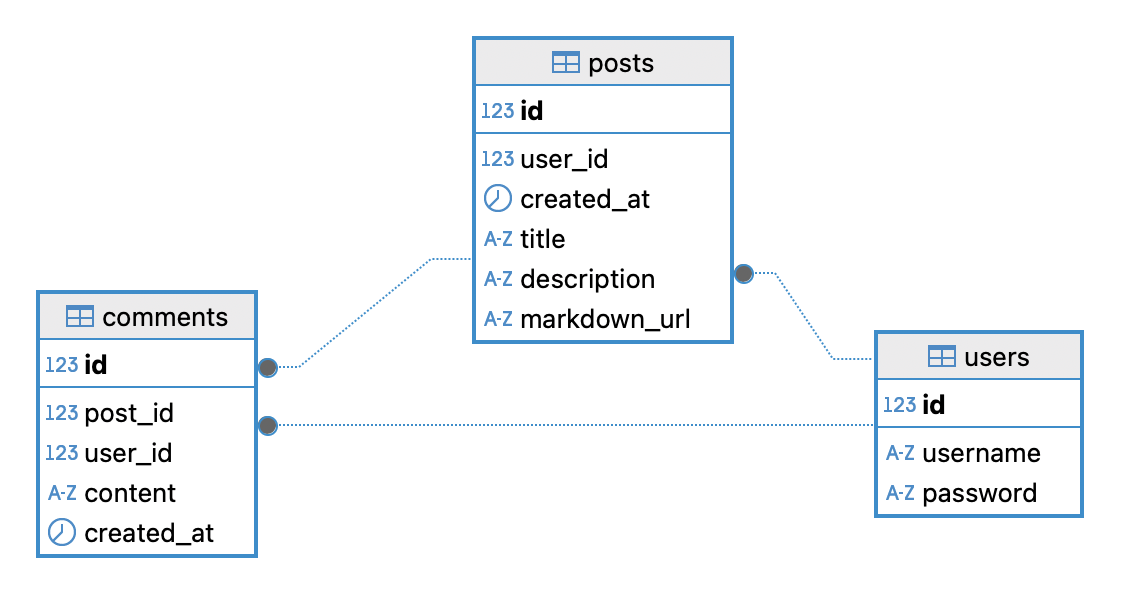
\includegraphics[width=12cm]{db-erd.png}
\centering
\caption{Database Entity Relationship Diagram}
\label{fig:db-erd}
\end{figure}

Information about each user needs to be stored, so a user table is naturally required. This includes any information about the user, such as username and password hash.
In the MVP of Omni, there is not much additional information stored about each user, but we could feasibly expand to store much more data for new features, such as storing a user's birthday.
In the future, if a hybrid approach for database distribution is used, a separate table to hold authentication data may be better to store this on a replicated database cluster rather than a sharded one.

The second easy-to-see table holds information about each post. It must store the creator's ID, title, description, link to the markdown file, timestamp, and more.
Posts will have a one-to-many relationship with users, where one user may create many posts, but each post is always associated with just one user. 

The final table is not as obvious to spot but still crucial: a table to store comments in. Storing this in the posts table does not make sense in a structured SQL database.
Adopting this approach could work in a NoSQL setup, but for popular posts, the document size would grow too big and slow down reading the post for everybody.
By storing the comments in a separate table, we can use pagination in our SQL queries to limit the number of comments we return to a user simultaneously.
This limits the load on the microservices, ensuring they are not overwhelmed by a very popular post with many comments.

\subsection{Discussion on Sharding}
As discussed in Section \ref{sec:design-system-database}, the design of the database and Snowflake IDs enable easy sharding of the database, whilst maintaining fast access times by backend microservices.
A single database has been used to maintain simplicity for the initial implementation and testing of the platform. The only difference this has in the code is that the logic for selecting which database node to retrieve data from is removed (as only one node contains all data).


\section{Backend Microservices}
\label{sec:impl-backend}
This section discusses how the backend microservices were created and how they interact with the broader environment.
Some patterns have been shared across services to enable as much code reuse as possible.

\subsection{Database Access}
\label{sec:impl-backend-db}
All three backend services require some level of database access. OmniAuth and OmniRead require only read access, whereas OmniWrite will read and write data. 

All the applications (currently) interact with the same database, although, as mentioned in Section \ref{sec:design-system-database-implementation}, future improvements could include using separate databases for things like authentication.
Because the database is shared, we can utilise the same database layer in each application, reducing the amount of code we need to write.

\subsubsection{The SQLc Library}
\underline{\href{https://sqlc.dev}{SQLc}} \nocite{sqlc} has been used to generate the database layer automatically.
This code generation library takes as input database migrations and all the queries to be run against the database.
It then compiles these inputs into type-safe code. There are multiple benefits to this approach:
\begin{itemize}
    \item Most of the code generated is boilerplate developers must write by hand or copy from documentation. It does not solve novel problems.
    \item The code generated is type-safe and handles embedding objects from joins for a more traditional object-orientated programming style. 
    \item The compiler flags breaking changes to the database via migrations when the database layer has been regenerated, but the business logic has not yet been modified.
\end{itemize}
Using this approach, SQLc has generated objects for users, posts, and comments, as well as other objects used when retrieving smaller data sections from each table.
Helpfully, the library generates an interface used within the code to access the database and an implementation of the interface for accessing the database.
However, this interface enables developers to write custom implementations, for example, to be used during unit testing. 

All the backend services share this database layer as there is no need to write the queries separately for each one, as operations like retrieving a user profile happen in all the services.

\subsubsection{Managing Database URLs}
In order for the services to make calls to the database, they need to know where to send requests.
This is defined by a URL that is passed to each application through the environment, allowing for on-the-fly changes to the configuration without having to rebuild each application. 
The start-up function parses this URL and then creates a database connection using Go's built-in \underline{\href{https://pkg.go.dev/database/sql}{database/SQL}} \nocite{gosqlpkg} package.
Finally, a Querier object (generated by SQLc) is initialised from the database connection object. This is the object which will be passed to each service's business logic so that database requests can be made.
